\section{Discussion}

We processed our data by transforming hexadecimal encoded byte values into numerical valued between 0 and 255 (unsigned bytes) as well as all the bit flags present in our flame detector units under test. We isolated two files (Test45.log, Test48.log) and a further representative section within these files, representing signal (fire) and noise (interference). Both sets of data plotted as Flame A detector, Flame B detector and Guard as discussed in Jupyter Notebook.

\subsection{Signal data}

We plotted our signal data finding that the fire event generated values for Flame Detector A and Flame detector B that closely overlapped.

\begin{figure}[tb]
 \centering % avoid the use of \begin{center}...\end{center} and use \centering instead (more compact)
 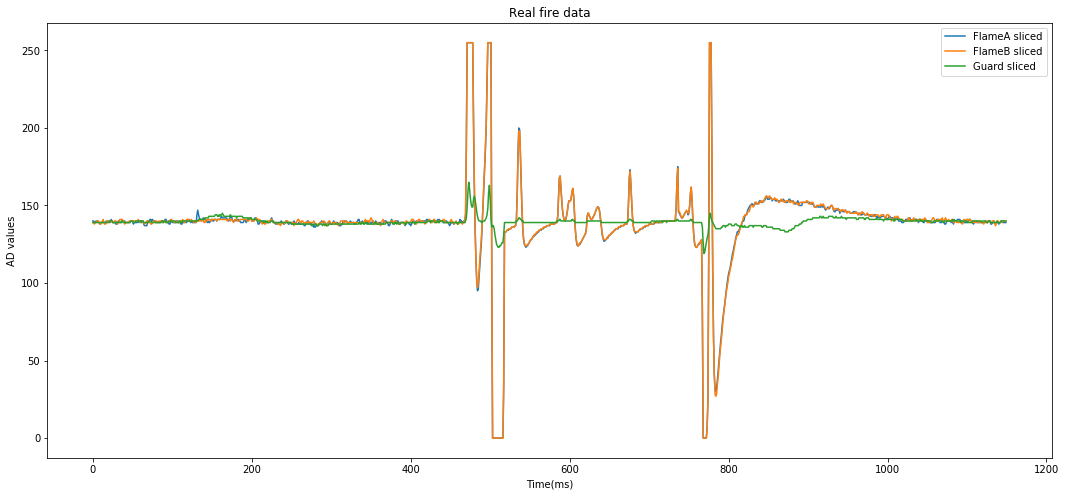
\includegraphics[width=\columnwidth]{pictures/01-real-fire-data.png}
 \caption{Closely overlapping Flame A and Flame B fire data}
 \label{fig:sample}
\end{figure}

\subsection{Noise data}

We plotted the same section of our noise data and found that Flame A and Flame B did not overlapped, in fact in parts they were going in opposite directions (antiphase), finding that this could become an engineered feature.

\begin{figure}[tb]
 \centering % avoid the use of \begin{center}...\end{center} and use \centering instead (more compact)
 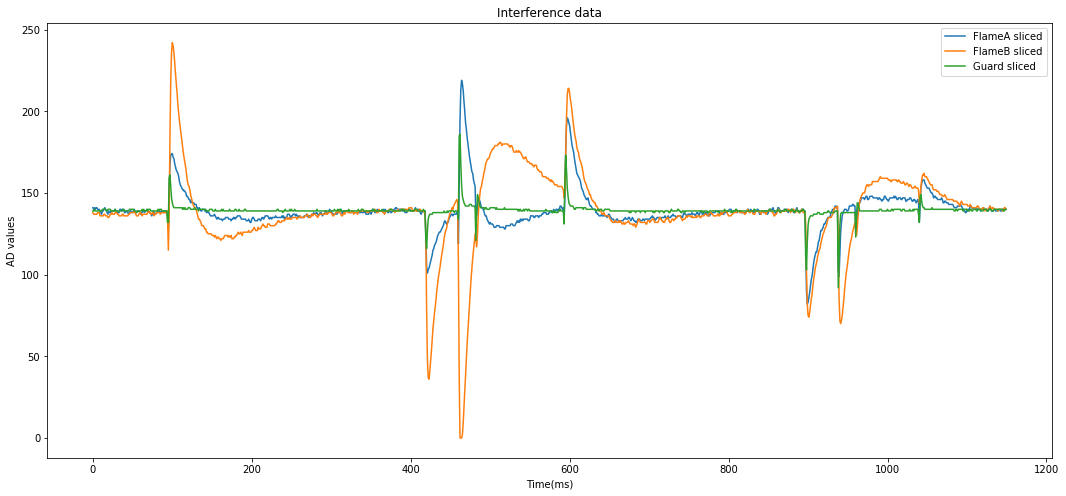
\includegraphics[width=\columnwidth]{pictures/02-interference-data.png}
 \caption{Interference plot, Flame A and Flame B with little or no overlap}
 \label{fig:sample}
\end{figure}

\subsection{Data normalisation}

We normalised our data, initially using a per-attribute minimum and maximum values:

$$ z{_i}=\frac{x{_i}-min(x)}{max(x)-min(x)} ,max(x)-min(x) \neq 0 $$

And found that this approach distorted our plot.

\begin{figure}[tb]
 \centering % avoid the use of \begin{center}...\end{center} and use \centering instead (more compact)
 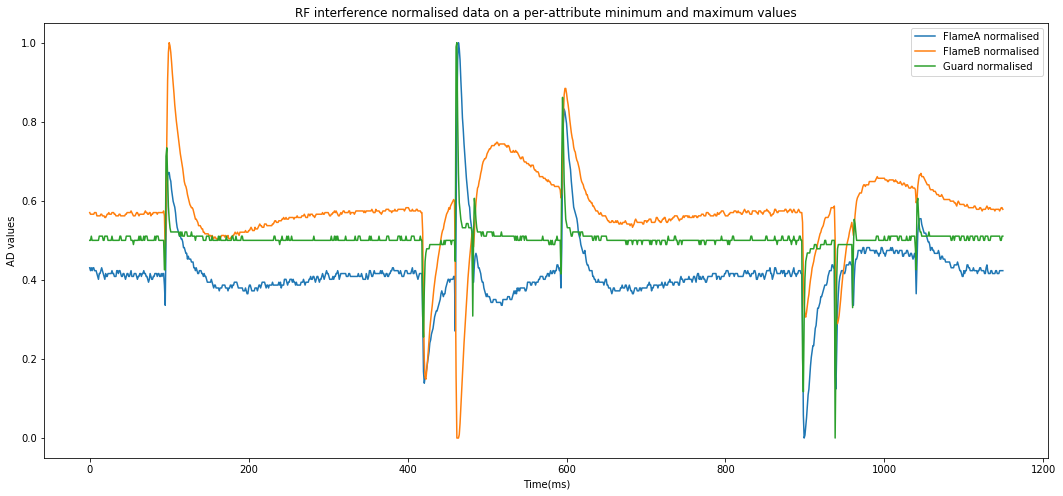
\includegraphics[width=\columnwidth]{pictures/03-interference-data-normalised-per-attribute-min-max.png}
 \caption{Normalised plot with distortion, per attribute minimum and maximum values}
 \label{fig:sample}
\end{figure}

So we modified the normalisation algorithm using minimum and maximum values across all attributes as they are scaled to same values (0-255)

$$ z{_i}=\frac{x{_i}-min}{max-min} , max-min \neq 0 $$

\subsection{Distance function}

Once our data was normalised, we created a distance function expecting that this would provide a measure to distinguish noise from signal. This approach was based on the degree of overlapping presented by Flame A and Flame B signals for fire data and inteference data. we obtained the distance value by the absolute difference of Flame A and Flame B

$$ Fd = |Nfa - Nfb| $$

With this engineered attribute we plotted both features to find that interference data presented, as expected, greater distances and fire data.

\begin{figure}[tb]
 \centering % avoid the use of \begin{center}...\end{center} and use \centering instead (more compact)
 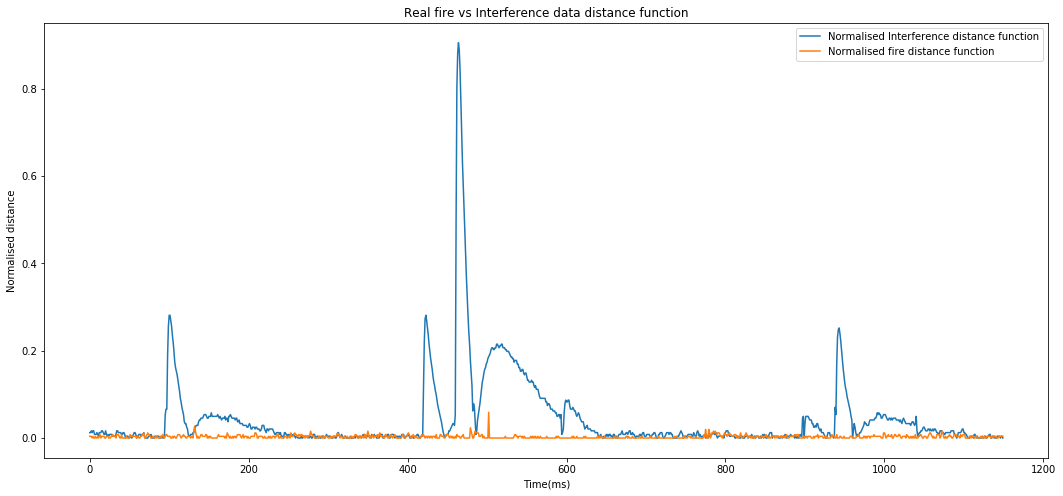
\includegraphics[width=\columnwidth]{pictures/06-fire-interference-distance-function.png}
 \caption{Fire and interference distance function}
 \label{fig:sample}
\end{figure}

\subsection{Linear regression}

Since the distance function showed how closely the signals of Flame A and Flame B were match, we figured it would be a good idea to plot our data plus a line of best fit, to confirm our findings using a well established approach.  
The interference data proved to have a weak positive correlation, while the fire data proved to have a strong positive correlation.

\begin{figure}[tb]
 \centering % avoid the use of \begin{center}...\end{center} and use \centering instead (more compact)
 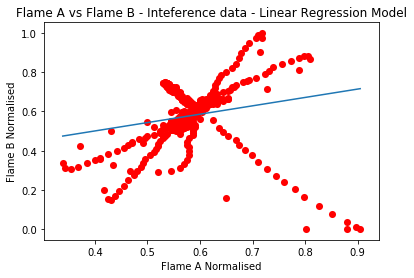
\includegraphics[width=\columnwidth]{pictures/07-interference-linear-regression.png}
 \caption{Interference linear regression - weak positive correlation}
 \label{fig:sample}
\end{figure}

\begin{figure}[tb]
 \centering % avoid the use of \begin{center}...\end{center} and use \centering instead (more compact)
 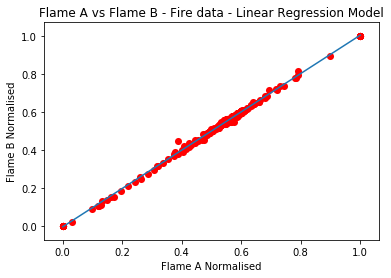
\includegraphics[width=\columnwidth]{pictures/08-fire-linear-regression.png}
 \caption{Fire data linear regression - strong positive correlation}
 \label{fig:sample}
\end{figure}

\subsection{Antiphase}

Our second and last engineered function was the antiphase flag, that is true whenever Flame A and Flame B signals are moving in opposite directions. This can be determined by dividing the deltas and verifying the sign, if it is found to be negative, the signals are in antiphase.

$$  A \Rightarrow \frac{\Delta Fa}{\Delta Fb}<0$$
where
$$ \Delta Fa = Fa{_i}-Fa{_{i-1}}, \Delta Fb = Fb{_i}-Fb{_{i-1}}, \forall i > 1 $$

With the antiphase attribute we were able to overlay this new attribute with the original plots. This showed us that interference data showed antiphase signals throughout the plot while fire data showed no antiphase in the fire signal section, suggesting that Flame A and Flame B were tightly overlapped.

We did notice however that the antiphase flag was not set throughout signals that visually appeared to be moving in opposite directions, this suggested there is further scope for improvement in the antiphase algorithm, perhaps using a window as in an interval of values, instead of discreet values, and this could be carried out in future works.

\begin{figure}[tb]
 \centering % avoid the use of \begin{center}...\end{center} and use \centering instead (more compact)
 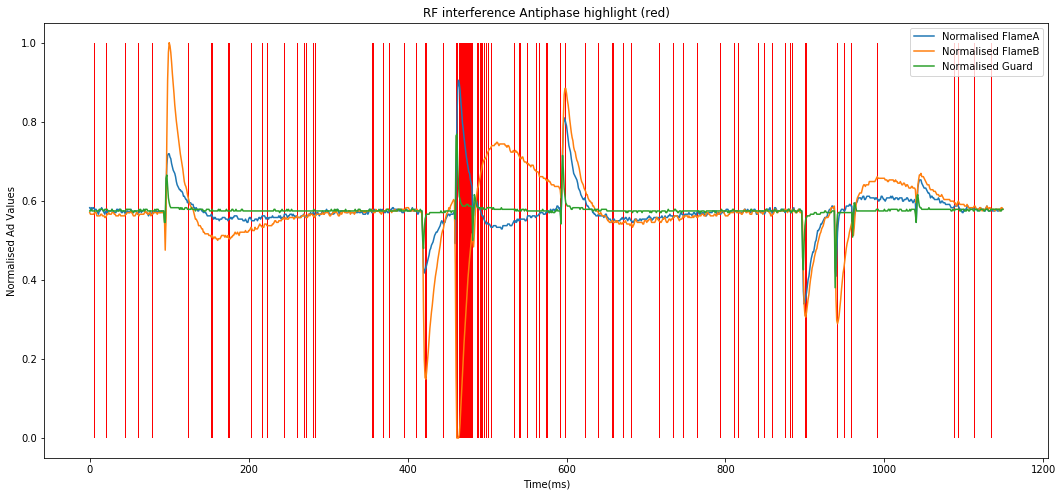
\includegraphics[width=\columnwidth]{pictures/09-interference-antiphase.png}
 \caption{Interference antiphase highlight (red)}
 \label{fig:sample}
\end{figure}

\begin{figure}[tb]
 \centering % avoid the use of \begin{center}...\end{center} and use \centering instead (more compact)
 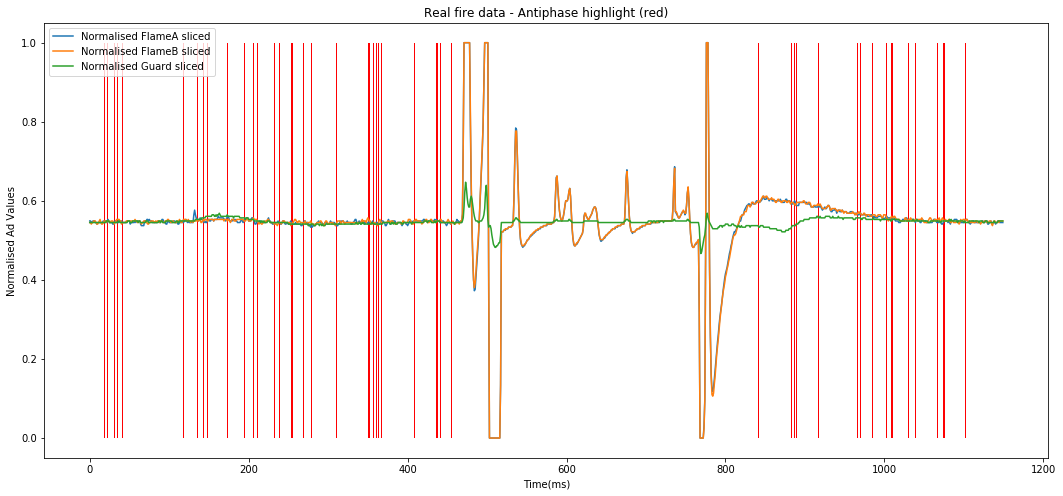
\includegraphics[width=\columnwidth]{pictures/10-fire-antiphase.png}
 \caption{Fire antiphase highlight (red)}
 \label{fig:sample}
\end{figure}


Between our distance function and antiphase function, we believe there is enough data to safely distinguish signal and noise which would have commercial applications in ensuring equipment would pass security integrity level approval tests. 

In addition to our engineer attributes, we also attempted fast fourier transforms which did not provide clear pointers, in this instance, as to the usefulness of the approach.

We first transformed noisy data obtaining a frequency plot, then replotted with data smoothed using the Savistzky-Golay filter, and found the frequency showed more regularity, by the increased number of zero crossing observed.

We then plotted the data with no filter applied, which showed a slightly noisier signal as expected, then the same data with a filter applied with is slightly smoother.

\begin{figure}[tb]
 \centering % avoid the use of \begin{center}...\end{center} and use \centering instead (more compact)
 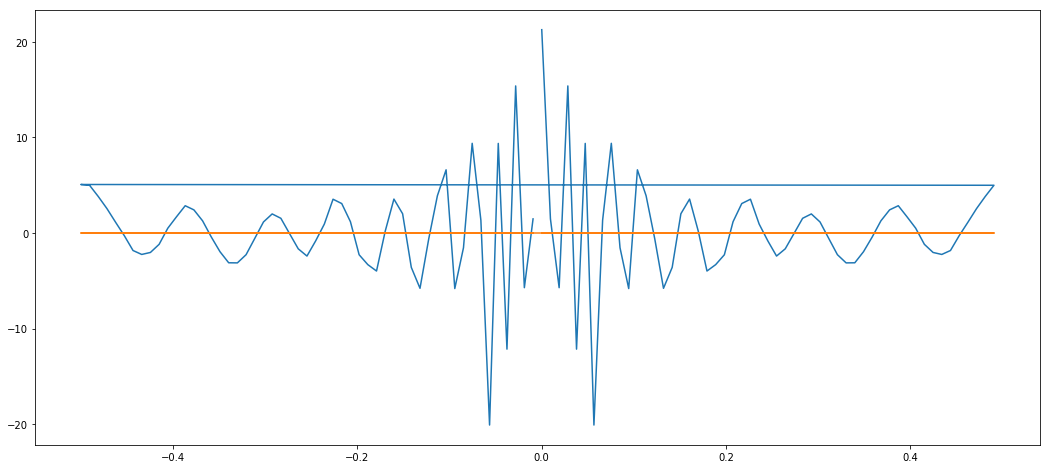
\includegraphics[width=\columnwidth]{pictures/15-inteference-slice-smoothed-fft.png}
 \caption{Interference slice smoothed fast fourier transform}
 \label{fig:sample}
\end{figure}
